\section{Results}
The following section presents the results of the user study. We examined perceived understanding, self-reported trust and an implicit trust measure via the willingness to follow a classifier's recommendation. For each topic, we give the mean score, standard deviation, as well as a comparison of all conditions in a 9x9 matrix.\newline
The matrices show each condition checked for significant difference with every other condition. The colour scale is a visualisation of the differences in means ($\bar{x}_{row} - \bar{x}_{column}$ ), with negative differences coloured in red and positive differences in green. Per cell, the net difference values are displayed as well. The significance test results are added with asterisks, where one asterisk means significant at $\alpha=0.05$ significance level, while two asterisks denote significance at $\alpha=0.01$ significance level.\newline 

\paragraph{Demographics}
In total, 327 participants took part in the main user study with an average age of 29.4 years (SD = 8.8), a gender balance of 56\% (females) to 43\% (males) and two participants reporting the third gender. 87\% of the participants were recruited via ``Prolific", while 36 participants enlisted on ``SurveyCircle". 57\% self-assessed their level of English to be equivalent to a native speaker, 23\% as advanced (C1), 14\% as upper-intermediate (B2), and 5\% as lower than that. All participants claimed to be ``fluent" in English. The exclusion criteria (passed attention check and completion of whole questionnaire) invalidated 41 data points, resulting in 286 valid cases. More detailed statistics about the participants' backgrounds are given in appendix B.\newline

\paragraph{Perceived Understanding}
As figure \ref{fig:results_matrix_understanding} shows, users of the system with a very good classifier and no explanation report the highest perceived understanding. For the very good and the medium classifier, giving no explanations for the decisions leads to a higher perceived understanding than delivering placebic, i.e. random, explanations. In general, users have more confidence in their understanding of the system for the very good and medium classifiers as compared to the bad classifier. One condition, however, does not lead to significantly higher scores than the bad classifier: for the medium classifier with random explanations, users reported the same understanding as for the bad classifier with no explanations. Concerning the bad classifier, giving a truthful explanation for the decision leads to the lowest perceived understanding.

\begin{table}[h]
	\makebox[\textwidth][c]{
	\begin{tabular}{lrr|lrr|lrr}
		\textbf{Condition} & \textbf{Mean} & \textbf{SD} & \textbf{Condition} & \textbf{Mean} & \textbf{SD} & \textbf{Condition} & \textbf{Mean} & \textbf{SD} \\ \midrule
		super-good & 3.944 & 0.915 & super-rand & 3.729 & 0.860 & super-no & 4.147 & 0.701 \\
		medium-good & 3.818 & 0.825 & medium-rand & 2.944 & 0.963 & medium-no & 3.700 & 0.690 \\
		bad-good & 2.465 & 1.201 & bad-rand & 2.500 & 1.138 & bad-no & 2.944 & 1.152 \\ \bottomrule
	\end{tabular}}
	\caption{Mean scores for perceived understanding measure}
	\label{fig:results_table_understanding}
\end{table}

\begin{figure}[H]
	\makebox[\textwidth][c]{
		\begin{minipage}[t]{0.65\textwidth}
			\centering
			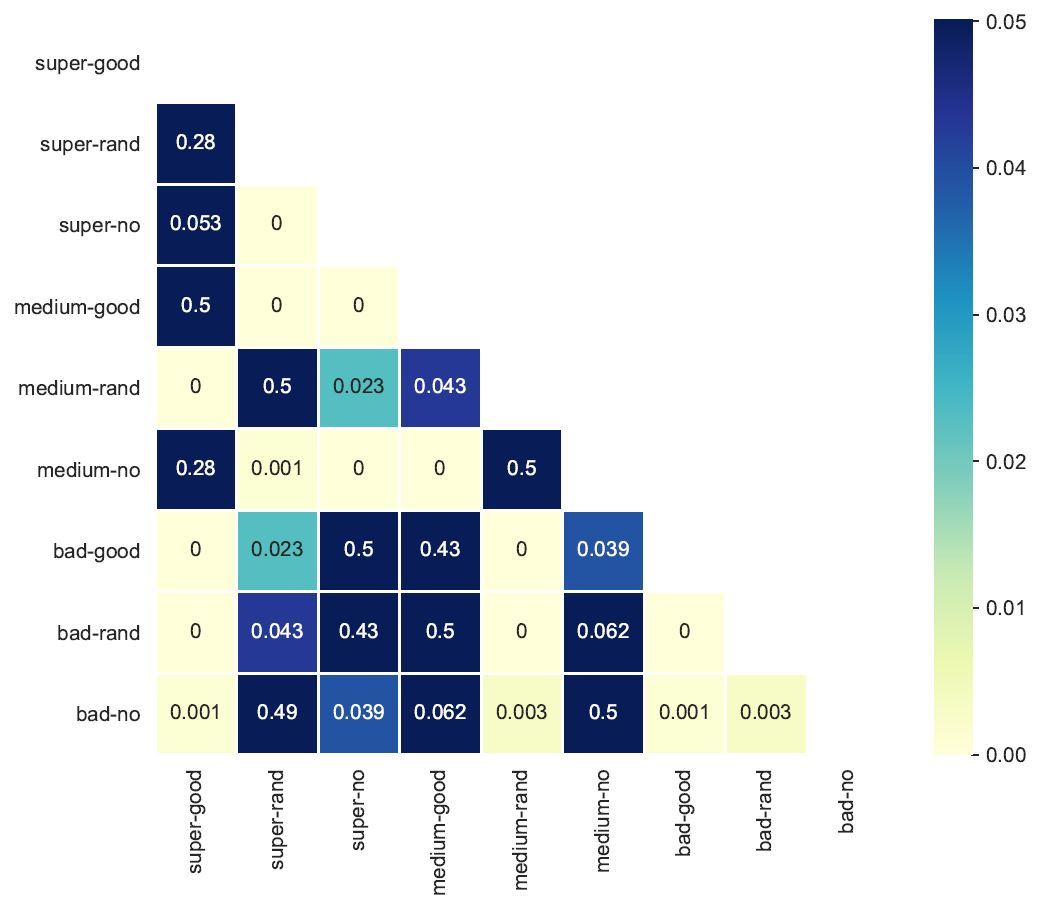
\includegraphics[width=\textwidth]{img/results_matrix_understanding.JPG}
			\caption{Comparison of perceived understanding scores ordered by classifier, value reporting difference of means ($\bar{x}_{row} - \bar{x}_{column}$ ), asterisk reporting significance (* significant at $\alpha=0.05$, ** significant at $\alpha=0.01$)}
			\label{fig:results_matrix_understanding}
		\end{minipage}%
		\hspace{5mm}
		\begin{minipage}[t]{0.65\textwidth}
			\centering
			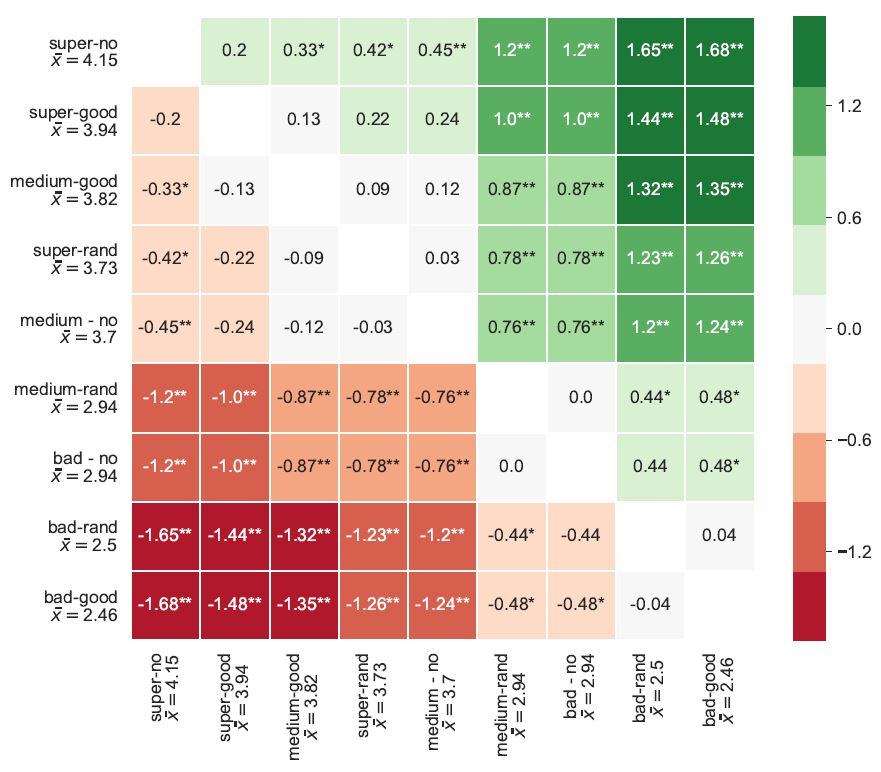
\includegraphics[width=\textwidth]{img/results_matrix_understanding_reordered.JPG}
			\caption{Comparison of perceived understanding scores ordered by explanation type, value reporting difference of means ($\bar{x}_{row} - \bar{x}_{column}$ ), asterisk reporting significance (* significant at $\alpha=0.05$, ** significant at $\alpha=0.01$)}
			\label{fig:results_matrix_understanding_reordered}
		\end{minipage}}
\end{figure}


\paragraph{Trust Questionnaire}
The self-reported trust scores show similar results as the perceived understanding: Besides the medium classifier with random explanations, all systems lead to significantly more trust than the systems employing the bad classifier. The explanations do not play a role regarding user's trust when the bad classifier is used. Looking at the medium classifier, the random explanation leads to a lower trust score than no explanation and a good explanation, with no difference between the latter two. The most trust is evoked by the very good classifier without explanations, significantly more than for any other condition. There is no significant difference between the very good classifier with explanations and the medium classifier with meaningful explanation. For both the bad classifier and the very good classifier, the condition without any explanation again led to the highest scores within the same classifiers. The detailed results are presented in figure \ref{fig:results_matrix_trust}.

\begin{table}[h]
	\makebox[\textwidth][c]{
		\begin{tabular}{lrr|lrr|lrr}
			\textbf{Condition} & \textbf{Mean} & \textbf{SD} & \textbf{Condition} & \textbf{Mean} & \textbf{SD} & \textbf{Condition} & \textbf{Mean} & \textbf{SD} \\ \midrule
			super-good & 2.682 & 0.400 & super-rand & 2.679 & 0.482 & super-no & 2.995 & 0.512 \\
			medium-good & 2.633 & 0.482 & medium-rand & 2.211 & 0.509 & medium-no & 2.630 & 0.459 \\
			bad-good & 1.917 & 0.428 & bad-rand & 1.951 & 0.403 & bad-no & 2.018 & 0.546 \\ \bottomrule
	\end{tabular}}
	\caption{Mean scores for self-reported trust measure}
	\label{fig:results_table_trust}
\end{table}

\begin{figure}[H]
	\makebox[\textwidth][c]{
		\begin{minipage}[t]{0.65\textwidth}
			\centering
			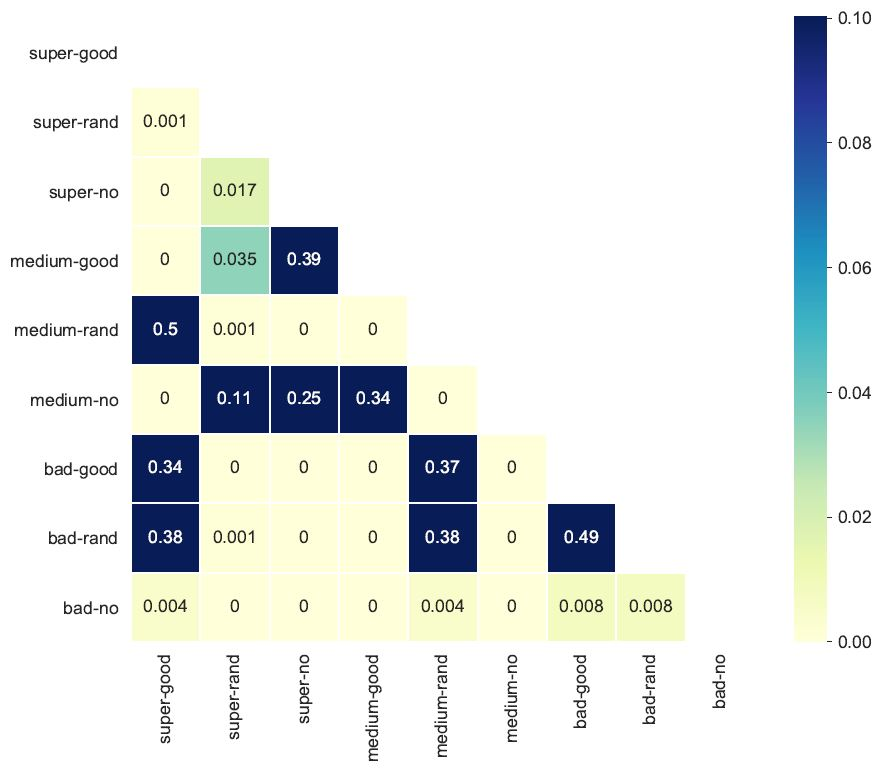
\includegraphics[width=\textwidth]{img/results_matrix_trust.JPG}
			\caption{Comparison of trust scores ordered by classifier, value reporting difference of means ($\bar{x}_{row} - \bar{x}_{column}$ ), asterisk reporting significance (* significant at $\alpha=0.05$, ** significant at $\alpha=0.01$)}
			\label{fig:results_matrix_trust}
		\end{minipage}%
		\hspace{5mm}
		\begin{minipage}[t]{0.65\textwidth}
			\centering
			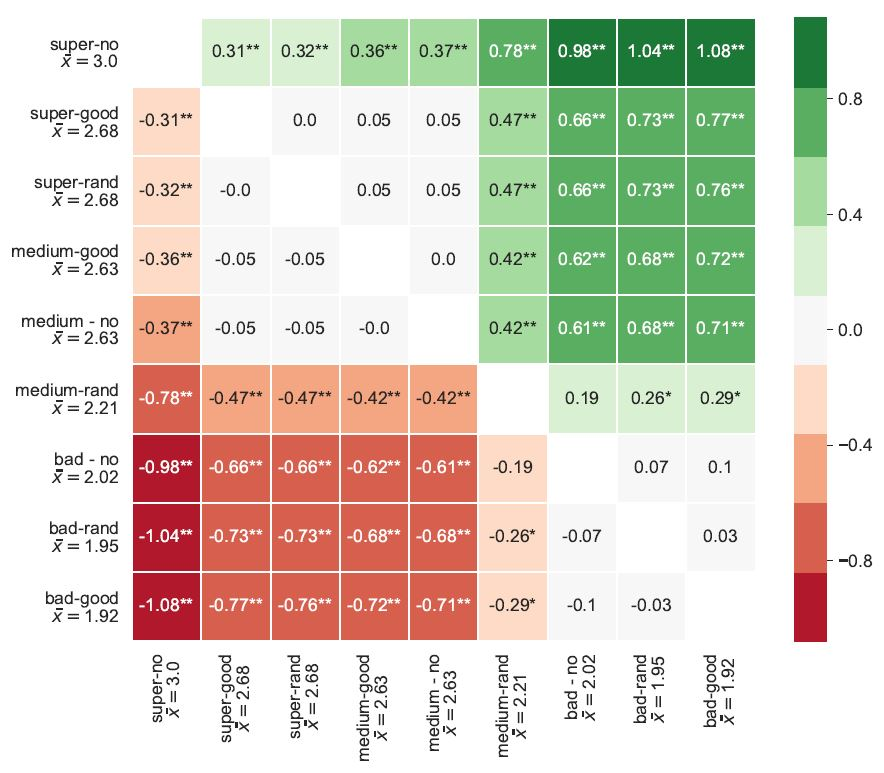
\includegraphics[width=\textwidth]{img/results_matrix_trust_reordered.JPG}
			\caption{Comparison of trust scores ordered by explanation type, value reporting difference of means ($\bar{x}_{row} - \bar{x}_{column}$ ), asterisk reporting significance (* significant at $\alpha=0.05$, ** significant at $\alpha=0.01$)}
			\label{fig:results_matrix_trust_reordered}
	\end{minipage}}
\end{figure}


\paragraph{Observed Trust via Proxy}
The second trust measure uses a proxy to determine the trust a user puts into a system: the willingness to follow a system's recommendation, in this case the decision about offensiveness and non-offensiveness. Figure \ref{fig:results_proxy_away} shows the results of analysing the user's willingness to change a classification to match the system's decision while contradicting the truth. As a comparison, figure \ref{fig:results_proxy_towards} deals with changes in classification that were made in favour of both the system and the truth.\newline
The results presented in this section need to be analysed with caution. Consider the case of the very good classifier with meaningful explanations. Out of 30 cases in this condition, 16 did not have the possibility to show a change away from the truth towards the prediction of the classifier, because the classifier in those 16 cases did not make any mistakes. From the remaining 14 cases, 4 showed the behaviour in question, leading to a mean of 0.286. This result is rather high, compared to the other conditions' mean scores. The same issue appears in the data for changing from a faulty classification towards a correct classification in accordance with the bad classifier: Each participant in this condition had at maximum once the possibility to show the behaviour in question. Seen that the number of participants in each group is not large to begin with, which is then reduced by the number of cases where such behaviour is not possible, the remaining sample size is very small for solid statistical analysis.\newline
The highest changing rate in favour of the system but against the true label was detected for users of the very good classifier with a meaningful explanation, but also the highest variance. Users were significantly more likely to adapt the system's faulty decision when confronted with the very good system with random and no explanations than the users of any system with the bad classifier. The same holds true for users of the medium classifier without explanations.\newline


\begin{table}[H]
	\makebox[\textwidth][c]{
		\begin{tabular}{lrrrrrrrr}
			\textbf{Condition} & 
			\head{1.5cm}{\textbf{Total cases}} & 
			\head{1.5cm}{\textbf{Cases with opportunities}} & 
			\head{1.5cm}{\textbf{Avg opportunities}} & 
			\head{1.5cm}{\textbf{Cases with changes}} & 
			\head{1.5cm}{\textbf{Avg changes}} & 
			\head{1.5cm}{\textbf{Cases with changes away}} & 
			\head{1.5cm}{\textbf{Avg changes away}} & 
			\head{1.5cm}{\textbf{Norma-lised mean}} \\ \midrule
			super-good &	30 &	 14 &	 0.47 &	 20 &	 1.40 &	 4 &	 0.29 &	 \textbf{0.29} \\
			super-rand &	32 &	 17 &	 0.53 &	 18 &	 1.09 &	 2 &	 0.12 &	 \textbf{0.12} \\
			super-no &	 	34 &	 23 &	 0.68 &	 18 &	 1.18 &	 1 &	 0.04 &	 \textbf{0.04} \\ 
			medium-good &	33 &	 33 &	 3.48 &	 17 &	 1.12 &	 7 &	 0.30 &	 \textbf{0.09} \\
			medium-rand &	30 &	 30 &	 3.57 &	 20 &	 1.37 &	 7 &	 0.30 &	 \textbf{0.08} \\
			medium-no &	30 &	 30 &	 3.40 &	 	20 &	 1.00 &	 5 &	 0.23 &	 \textbf{0.08} \\
			bad-good &	 	38 &	 38 &	 14.45 &	 20 &	 0.95 &	 17 &	 0.71 &	 \textbf{0.05} \\
			bad-rand &	 	30 &	 30 &	 14.27 &	 19 &	 1.13 &	 15 &	 0.77 &	 \textbf{0.05} \\
			bad-no &	 	30 &	 30 &	 14.27 &	 19 &	 1.23 &	 16 &	 1.03 &	 \textbf{0.07} \\ \bottomrule
	\end{tabular}}
	\caption{Statistics for trust measure via proxy (changes away from truth in favour of system decision)}
	\label{fig:results_table_proxy_away}
\end{table}

\begin{figure}[H]
	\makebox[\textwidth][c]{
		\begin{minipage}[t]{0.65\textwidth}
			\centering
			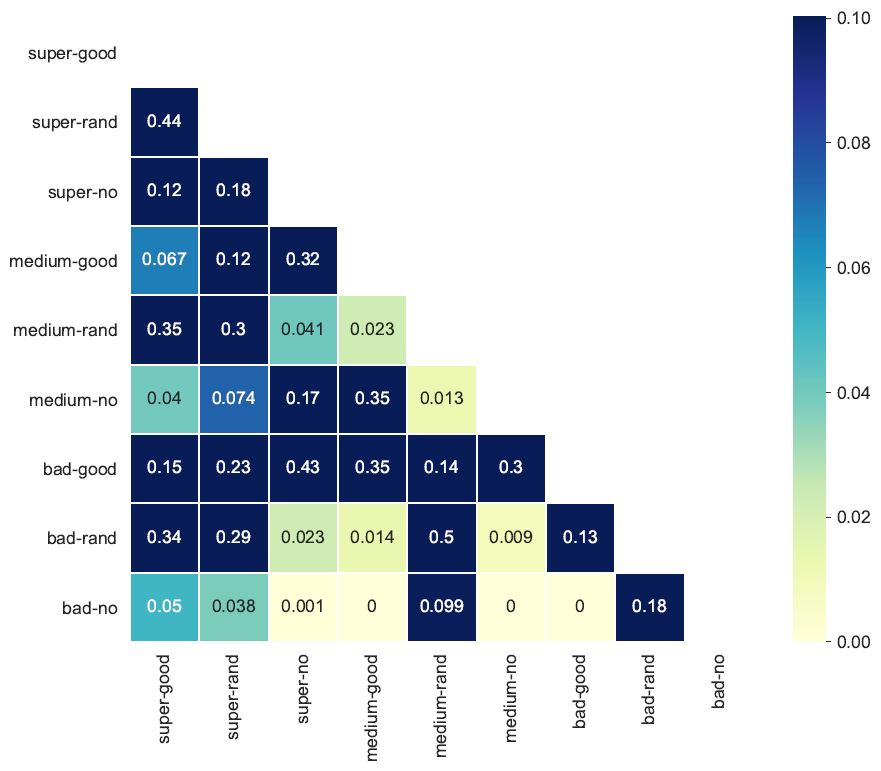
\includegraphics[width=\textwidth]{img/results_matrix_proxy_away.JPG}
			\caption{Comparison of proxy trust (away) scores ordered by classifier, value reporting difference of means ($\bar{x}_{row} - \bar{x}_{column}$ ), asterisk reporting significance (* significant at $\alpha=0.05$, ** significant at $\alpha=0.01$)}
			\label{fig:results_proxy_away}
		\end{minipage}%
		\hspace{5mm}
		\begin{minipage}[t]{0.65\textwidth}
			\centering
			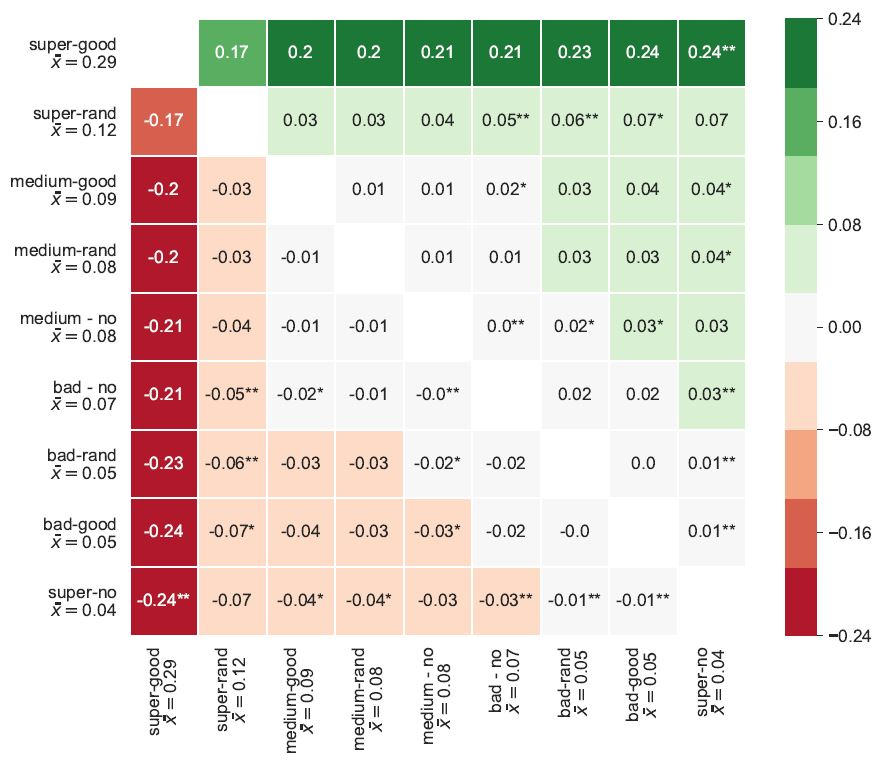
\includegraphics[width=\textwidth]{img/results_matrix_proxy_away_reordered.JPG}
			\caption{Comparison of proxy trust (away) scores ordered by explanation type, value reporting difference of means ($\bar{x}_{row} - \bar{x}_{column}$ ), asterisk reporting significance (* significant at $\alpha=0.05$, ** significant at $\alpha=0.01$)}
			\label{fig:results_proxy_away_reordered}
	\end{minipage}}
\end{figure}
\noindent Looking at the changes made towards the truth in agreement with the classifiers, no significant differences are noted between any condition with the very good and medium classifier. The same holds true for the bad classifier. The very good and medium classifiers, however, evoked significantly more changes towards the truth than the bad classifier with explanations. The standard deviations of the conditions using the bad classifier are rather high as compared to any other condition.\newline
One condition is exceptional in this analysis: Although the bad classifier without explanation has the highest mean score (i.e. changes towards the truth when the classifier made a correct prediction), the score is not significantly different from the bad classifier with a good and random explanation. The variance of all three systems (bad-no, bad-random, bad-good) are very high as compared to the variances of the other systems. The score deviates, however, from the results of the very good and medium classifier, which have lower mean scores but lower variances. The difference in variance is important to note when comparing the relatively high mean score of the bad classifier without explanation to the conditions with the very good and medium classifiers.

\begin{table}[H]
	\makebox[\textwidth][c]{
		\begin{tabular}{lrrrrrrrr}
			\textbf{Condition} & 
			\head{1.5cm}{\textbf{Total cases}} & 
			\head{1.5cm}{\textbf{Cases with opportunities}} & 
			\head{1.5cm}{\textbf{Avg opportunities}} & 
			\head{1.5cm}{\textbf{Cases with changes}} & 
			\head{1.5cm}{\textbf{Avg changes}} & 
			\head{1.5cm}{\textbf{Cases with changes towards}} & 
			\head{1.5cm}{\textbf{Avg changes towards}} & 
			\head{1.5cm}{\textbf{Norma-lised mean}} \\ \midrule
			super-good &	 30 &	 30 &	 14.53 &	 20 &	 1.40 &	 18 &	 1.07 &	 \textbf{0.07} \\
			super-rand &	 32 &	 32 &	 14.47 &	 18 &	 1.09 &	 14 &	 0.69 &	 \textbf{0.05} \\
			super-no &	 	34 &	 34 &	 14.32 &	 18 &	 1.18 &	 15 &	 0.91 &	 \textbf{0.06} \\
			medium-good &	 33 &	 33 &	 11.52 &	 17 &	 1.12 &	 12 &	 0.67 &	 \textbf{0.06} \\
			medium-rand &	 30 &	 30 &	 11.43 &	 20 &	 1.37 &	 12 &	 0.57 &	 \textbf{0.05} \\
			medium-no &	 30 &	 30 &	 11.60 &	 20 &	 1.00 &	 16 &	 0.67 &	 \textbf{0.06} \\
			bad-good &	 	38 &	 21 &	 0.55 &	 20 &	 0.95 &	 1 &	 0.05 &	 \textbf{0.05} \\
			bad-rand &	 	30 &	 22 &	 0.73 &	 19 &	 1.13 &	 1 &	 0.05 &	 \textbf{0.05} \\
			bad-no &	 	30 &	 22 &	 0.73 &	 19 &	 1.23 &	 2 &	 0.09 &	 \textbf{0.09} \\ \bottomrule
	\end{tabular}}
	\caption{Statistics for trust measure via proxy (changes towards truth and system decision)}
	\label{fig:results_table_proxy_towards}
\end{table}

\begin{figure}[H]
	\makebox[\textwidth][c]{
		\begin{minipage}[t]{0.65\textwidth}
			\centering
			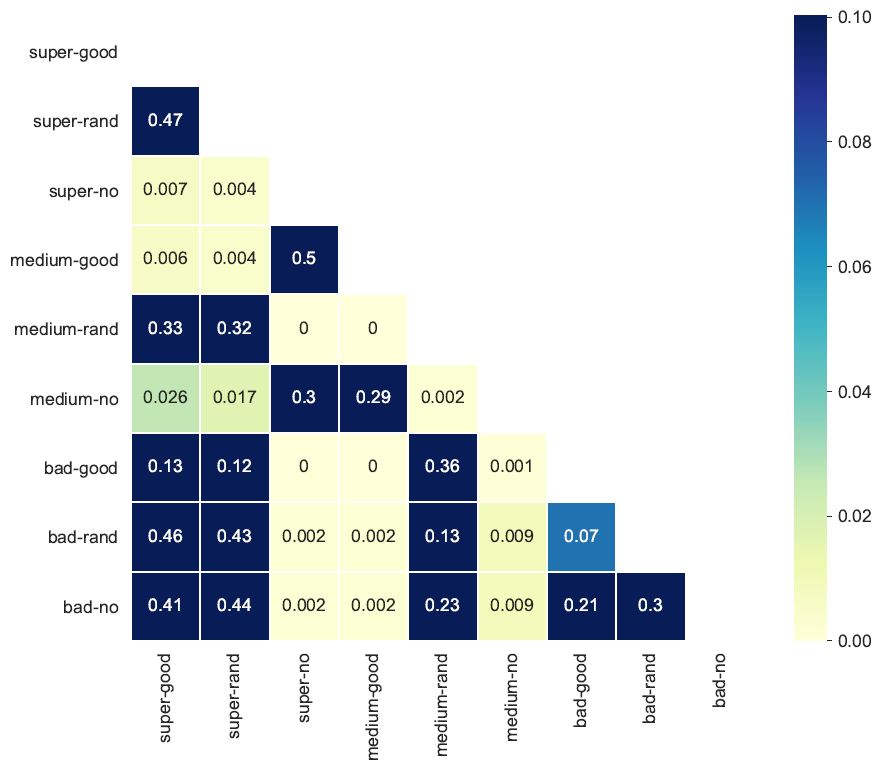
\includegraphics[width=\textwidth]{img/results_matrix_proxy_towards.JPG}
			\caption{Comparison of proxy trust (towards) scores ordered by classifier, value reporting difference of means ($\bar{x}_{row} - \bar{x}_{column}$ ), asterisk reporting significance (* significant at $\alpha=0.05$, ** significant at $\alpha=0.01$)}
			\label{fig:results_proxy_towards}
		\end{minipage}%
		\hspace{5mm}
		\begin{minipage}[t]{0.65\textwidth}
			\centering
			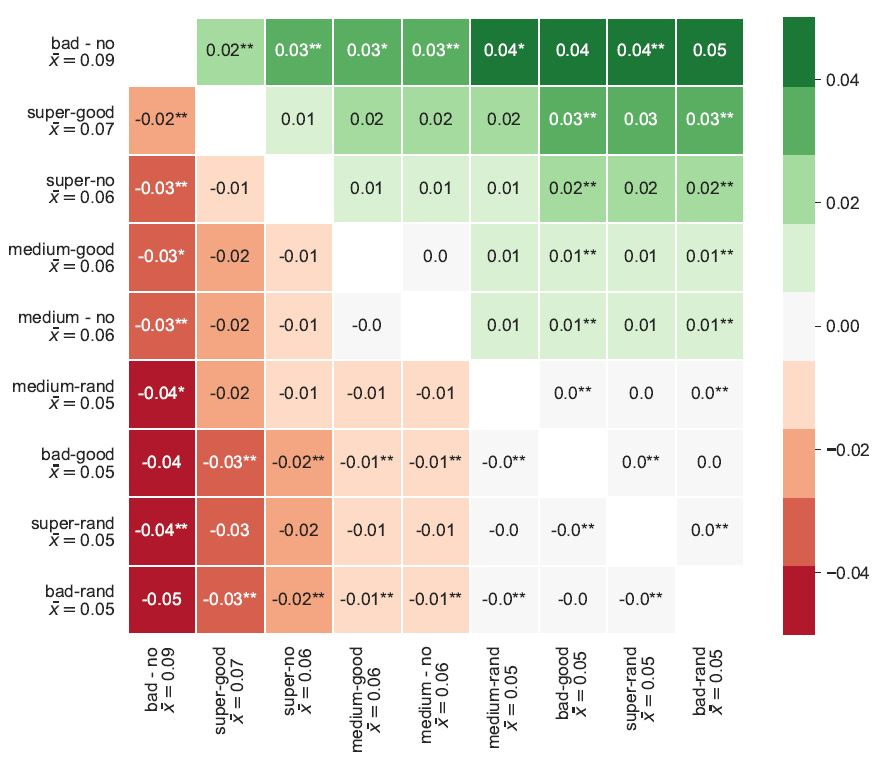
\includegraphics[width=\textwidth]{img/results_matrix_proxy_towards_reordered.JPG}
			\caption{Comparison of proxy trust (towards) scores ordered by explanation type, value reporting difference of means ($\bar{x}_{row} - \bar{x}_{column}$ ), asterisk reporting significance (* significant at $\alpha=0.05$, ** significant at $\alpha=0.01$)}
			\label{fig:results_proxy_towards_reordered}
	\end{minipage}}
\end{figure}

\paragraph{Observed Trust via Proxy}
The questionnaire used to measure self-perceived trust categorises six factors of trust. Although this research does not aim to investigate trust in more detail, we look at predictability in isolation, since we have two classifiers at the extremes which are predictable in their behaviour. Figure \ref{fig:results_matrix_predictability} and \ref{fig:results_matrix_predictability_reordered} show the results of comparing the predictability scores. The highest predictability was reported for \textit{super-no}, and the lowest for \textit{bad-rand}. All systems using the very good classifier are perceived to be significantly more predictable than the systems based on the bad classifier.
\begin{table}[h]
	\makebox[\textwidth][c]{
		\begin{tabular}{lrr|lrr|lrr}
			\textbf{Condition} & \textbf{Mean} & \textbf{SD} & \textbf{Condition} & \textbf{Mean} & \textbf{SD} & \textbf{Condition} & \textbf{Mean} & \textbf{SD} \\ \midrule
			super-good & 3.033 & 0.755 & super-rand & 2.914 & 0.814 & super-no & 3.213 & 0.725 \\
			medium-good & 2.864 & 0.594 & medium-rand & 2.308 & 0.833 & medium-no & 2.675 & 0.756 \\
			bad-good & 2.013 & 0.644 & bad-rand & 1.850 & 0.679 & bad-no & 2.117 & 0.763 \\ \bottomrule
	\end{tabular}}
	\caption{Mean scores for predictability}
	\label{fig:results_table_predictability}
\end{table}

\begin{figure}[H]
	\makebox[\textwidth][c]{
		\begin{minipage}[t]{0.65\textwidth}
			\centering
			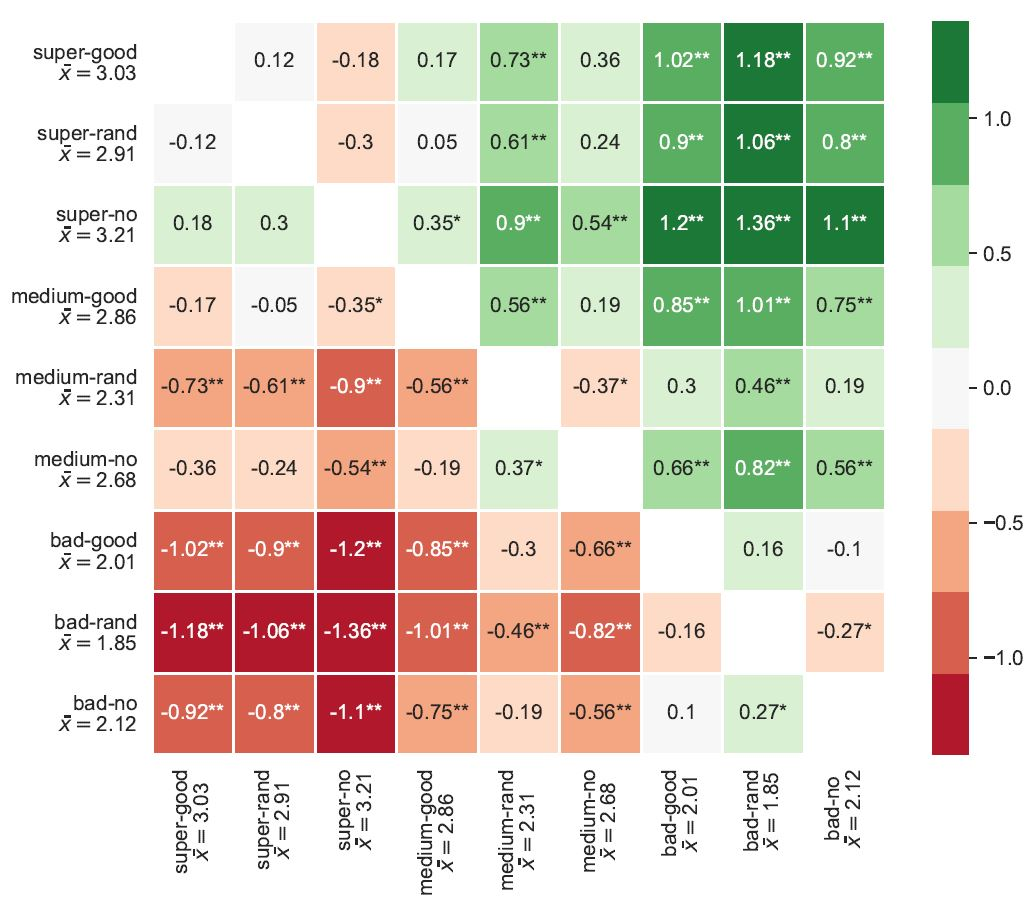
\includegraphics[width=\textwidth]{img/results_matrix_predictability.JPG}
			\caption{Comparison of predictability scores ordered by classifier, value reporting difference of means ($\bar{x}_{row} - \bar{x}_{column}$ ), asterisk reporting significance (* significant at $\alpha=0.05$, ** significant at $\alpha=0.01$)}
			\label{fig:results_matrix_predictability}
		\end{minipage}%
		\hspace{5mm}
		\begin{minipage}[t]{0.65\textwidth}
			\centering
			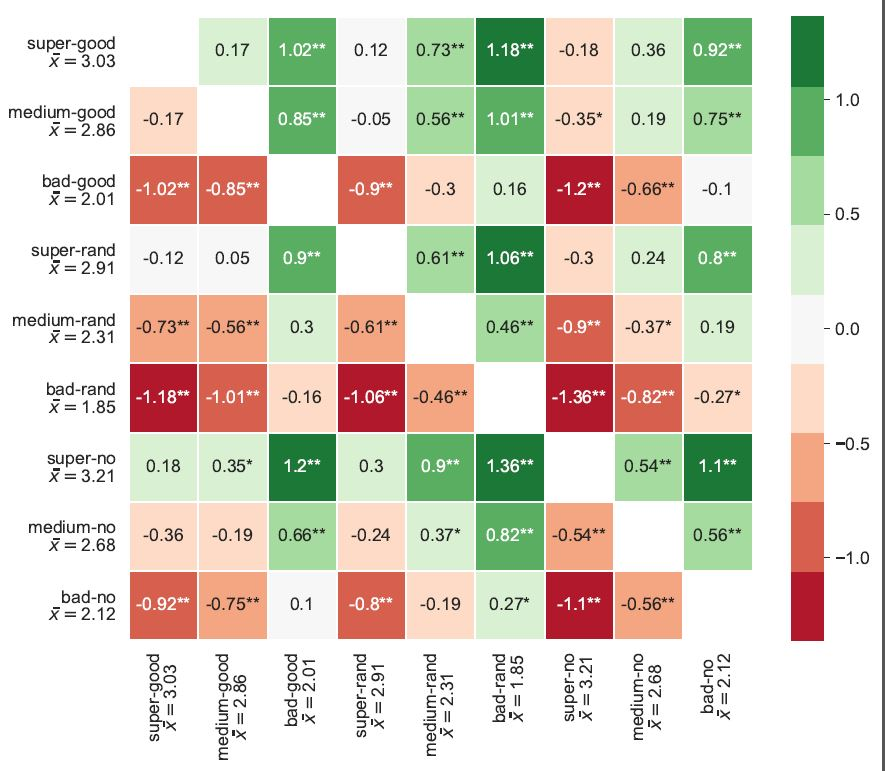
\includegraphics[width=\textwidth]{img/results_matrix_predictability_reordered.JPG}
			\caption{Comparison of predictability scores ordered by explanation type, value reporting difference of means ($\bar{x}_{row} - \bar{x}_{column}$ ), asterisk reporting significance (* significant at $\alpha=0.05$, ** significant at $\alpha=0.01$)}
			\label{fig:results_matrix_predictability_reordered}
	\end{minipage}}
\end{figure}




